%This document will explain the major features of the document
%class. For further information, the {\itshape \LaTeX\ User's Guide} is
%available from
%\url{https://www.acm.org/publications/proceedings-template}.
\documentclass[sigconf]{acmart}

\usepackage{lipsum}
\usepackage{pgfplots}
%Path relative to the .tex file containing the \includegraphics command
\graphicspath{ {images/} }

\begin{document}

\settopmatter{printacmref=false} % Removes citation information below abstract
\renewcommand\footnotetextcopyrightpermission[1]{} % removes footnote with conference information in first column
\pagestyle{plain} % removes running headers
\settopmatter{printfolios=true}


\title{libmicrovmi - The approach to unite the VMI ecosystems}
\author{Martin Johannes Loos}
\affiliation{\institution{University of Passau}}
\email{loos04@ads.uni-passau.de}


\begin{abstract}
Virtual machine introspection (VMI) enables the monitoring of virtual machines (VMs) at runtime from the outside.
In the current VMI application landscape, there are already some software solutions (e.g. pyvmidbg, PANDA, PyREBox, Drakvuf, icebox) but most of them have been developed especially for one hypervisor.
The reason for this is that there was no library with which one could develop independently of the underlying virtual machine monitor or emulator.
Libmicrovmi tries to solve exactly this problem by providing a low-level core library, which aims to be cross-platform, hypervisor-agnostic, and emulator-agnostic. Existing VMI applications or other higher-level API's can rebase on top of it.
In this paper, we present the core functionality of libmicrovmi. 
In addition, we also draw a comparison with the de facto standard VMI library libVMI.
Finally, we also analyze the performance of these two libraries in comparison for 3 different use cases (memory dump, register dump, CR3 event). We implemented this by executing these tasks with a Python program, which measures and logs the time required for this. In order to make a statistical evaluation possible, we obtained 100 measured values ​​for each task.
\end{abstract}

%%
%% Keywords. The author(s) should pick words that accurately describe
%% the work being presented. Separate the keywords with commas.
\keywords{libmicrovmi, virtual machine introspection}

\maketitle

\section{Introduction}
Virtual machine introspection (VMI) enables the monitoring of virtual machines (VM's) at runtime from the outside.
One main reason to use this is to observe a VM for suspicious activities from the outside, where it is harder to be detected.
\newline
\newline
As the successor of the XenAccess project, libVMI made a big impact for developing new virtual machine introspection applications. The primary reasons for this are replacing manual memory mapping with read and write functions and improving the overall performance of the library by using different caches \cite{payne2012simplifying}. We cover libVMI, besides other important background informations, in Chapter 2, because we will use it for comparison.
\newline
\newline 
With libmicrovmi \cite{githublibmicrovmi}, they took the next step to simplify the development of virtual machine introspection. It is a low-level VMI library which aims to be cross-platform, hypervisor-agnostic and emulator-agnostic. The goal of libmicrovmi is to unite the already existing VMI application ecosystem by providing an application programming interface (API) where all of them can rebase on. The core concepts are clarified in detail in Section 3.1.
\newline
\newline
To understand the similarities and differences between libmicrovmi and libVMI, we will discuss them in Section 3.2.
While libVMI is around and used for a while, libmicrovmi is relatively new. Therefore, we want to compare the performance of the two libraries in Section 3.3 in order to assess whether the performance of libmicrovmi is sufficient in practice or not. This is done through a statistical comparison of the runtimes for 3 different use cases.

\section{Background}
It requires some previous knowledge to understand the topic dealt with in this paper. In this chapter we explain these to an extent sufficient for a basic understanding. 
First, in Section 2.1 the core concepts of virtualization are explained. 
Second, in Section 2.2, the Xen hypervisor is covered with the most important concepts.
Third, we discuss in Section 2.3 what virtual machine introspection is, how it works, and why it is relevant.
Fourth, in Section 2.4 we explain a very popular VMI API called libVMI. We will use this in Chapter 3 for a comparison with libmicrovmi.
Finally, we discuss in Section 2.5 the basics of the programming language Rust in which libmicrovmi was programmed.
The main topic libmicrovmi is then covered in Chapter 3.

\subsection{Virtualization}
The concept of virtualization has been around for many years. At the beginning of work in this field in the 1960s and 1970s, the scope of this technology was completely different. The computing power, which has increased dramatically since then, has repeatedly resulted in new relevant fields of application \cite{graziano2011performance}. There are different types of virtualization.
In this paper we provide an overview of operating system virtualization in connection with the Xen hypervisor and its
paravirtualization architecture, which we cover in Section 2.2.
\newline
\newline
Operating system virtualization requires the use of system software between the guest operating system and the underlying hardware. This system software is known as a hypervisor or virtual machine monitor (VMM).
The hypervisor enables several operating systems to be used simultaneously on the same hardware.
Each operating system thinks that it is running on its own computer. The VMM is also responsible for managing and allocating the hardware resources.
\newpage
\begin{definition}
``Virtualization is the faithful reproduction of an entire architecture in software which provides the illusion of a real machine to all software running above it.'' \cite{kiyanclar2005survey}
\newline
\end{definition}

Gerald J. Popek and Robert P. Goldberg formulated requirements for virtualizable architectures in 1974 \cite{popek1974formal}. These requirements still provide a good assessment of whether a processor architecture can efficiently support virtualization.
\newline
\begin{itemize}
	\item Requirement 1: The execution of non-privileged instructions in privileged mode must be pretty much the same as in user mode.
	\newline 
	\item Requirement 2: There must be a mechanism that protects the real system and all other virtual machines from the active virtual machine.
	\newline
	\item Requirement 3: Always when a virtual machine tries to perform a sensitive instruction (instructions that interfere with the state of the underlying VMM or host OS) there must be a way to automatically signal this the VMM.
\newline
\end{itemize}

The third requirement ist the most important one for virtual machine introspection which we cover in Section 2.3. Whenever a sensitive instruction is executed by the virtual machine, the virtual machine monitor can investigate the state of the VM.
\newline
\newline
Garfinkel and Rosenblum described the crucial properties of the hypervisor in 2003 \cite{garfinkel2003virtual}:
\newline
\begin{itemize}
	\item Isolation: Everything that runs inside a virtual machine is isolated from the hypervisor and cannot corrupt the VMM or any other VM on the same physical machine.
	\newline 
	\item Inspection: The VMM can fully control the system state of a virtual machine. This makes it hard for an attacker to hide himself, because the hypervisor can see everything from outside the virtual machine.
	\newline
	\item Interposition: It is possible for the hypervisor to interpose the control flow of a virtual machine at specific virtual machine operations (e.g. performing privileged instructions).
	\newline
\end{itemize}

\subsection{Xen Hypervisor}
Xen is an open-source, bare-metal (Type I) hypervisor. It is currently available for the IA-32, x86-64 and ARM instruction sets. Some responsibilities of the Xen hypervisor are launching the privileged domain (virtual machine) dom0 at boot, CPU scheduling of the unprivileged virtual machines (domU's) and memory management. Dom0 is the only VM that has direct hardware access by default. It is also possible to create custom privileged domains who manage specified unprivileged domains \cite{7847045}. In our test environment at the cloud computing chair at the University of Passau we used this feature, because every student is in need for a seperated monitoring domain for his user domains (domU's).
\newline
\newline
Xen version 3.0 introduced the capability to run an unmodified guest operating system if the host machines processor supports hardware virtualization provided by Intel Virtualization Technology \cite{abels2005overview} or AMD-V. Xen will fall back to pure para-virtualization mode on unsupported hardware, allowing you to virtualize ``Xen aware'' guests on any hardware.
\newline
\newline
The following graphic shows a virtual machine host with three virtual machines. The Xen hypervisor is shown as running directly on the physical hardware platform. Note that the controlling domain is also a virtual machine, although it has several additional management tasks compared to all the other virtual machines.
\newline
\begin{figure}[h]
\centering
\includegraphics[width=0.5\textwidth]{xen-architecture}
\caption{Basic example of the Xen architecture}
\end{figure}
\newline
Dom0 is also known as the management and control domain. The reason for this is that the management and control software is being executed in it. It also contains the device drivers of all the managed domains and is permitted to use the control interface of the Xen hypervisor. With the control interface, other domains can be created and deleted. Also, the configuration of the domU's (e.g. scheduling parameters and physical memory allocation) are managed through it. Dom0 has access to the physical devices and provides virtual devices to domU's. The guest OS has to implement a front-end driver and the dom0 the back-end driver.


\subsection{Virtual Machine Introspection}
Virtual machine introspection enables the monitoring of a virtual machine at runtime. It looks at the main memory and the CPU registers of the monitored virtual machines to analyze their system states.
\newline
\begin{definition}
``We call this approach of inspecting a virtual machine from the outside for the purpose of analyzing the software running inside it virtual machine introspection (VMI).'' \cite{garfinkel2003virtual}
\newline
\end{definition}
There are various ways to monitor the state of a virtual machine. With an in-guest approach (e.g. anitvirus software) you only secure the operating system from threats, but this is very easily detectable and offers no isolation. Another way would be to scan the disk and the memory of the virtual machine, but then you have no interposition. With VMI, the protection of the VM is done from the outside (isolation). It also offers an effective way for monitoring and controlling (interposition). 
\newline
\newline
In comparison with other in-guest tracing techniques, VMI has the following security relevant properties:
\newline
\begin{itemize}
	\item Protection: Because of the isolation of the monitoring tool from the virtual machine, an attacker can not compromise the analyzing system directly.
	\newline 
	\item Stealthiness: Virtual machine introspection is hard to detect, because there is no need for monitoring software on the monitored virtual machine. 
	\newline
	\item Untampered View: Data which is collected through VMI can't be changed from an attacker in the analyzed system.
\newline
\end{itemize}

Virtual machine introspection can be carried out actively (synchronous) or passively (asynchronous) \cite{6956590}.
\newline
\newline
Synchronous mechanisms require the monitored VM to be paused. Trapped events are then transferred from the VM to the VMI application via the hypervisor. After the VMI application has processed the event, the VM can continue to run. As a result, the processing time has a direct impact on the monitored machine. In contrast to this, it is unnecessary to pause the monitored VM with asynchronous VMI. The introspection is done from a memory snapshot or from a read-only or copy-on-write view of the guest's memory. This means that there is no direct performance impact on the guest VM, but we may miss transient attacks.
\newline
\newline
To access raw memory and retrieve information out from it (interpretation), it must be known where and how an application stores it. Therefore, semantic knowledge of the data structure layout is needed to correctly identify information. This challenge in memory forensics is known as the semantic gap problem:
\newline
\begin{definition}
 ``The semantic gap is a challenge inherent in all applications of virtual machine introspection (VMI). It describes the disconnect between the low-level state that the hypervisor has access to and its semantics within the guest.'' \cite{schneider2012bridging}
\newline
\end{definition}

Virtual machine introspection has multiple advantages compared to memory forensics, which relies on a memory snapshot of a virtual machine. For example, it gives the possibility of tracing the execution of virtual machines. This is done by replacing non-sensitive instructions with sensitive instructions which then are being trapped by the CPU to the hypervisor. The virtual machine monitor can then intercept the control flow and analyze the state of the virtual machine. When finished, the original non-sensitive instruction is reinserted and the VM can continue running. This process needs to be done quickly. There are two main reasons for this. Firstly, the user of the virtual machine should not have to wait for the monitoring tasks of the VMM. Secondly, it is easier for malicious software to detect that a VMM trapped the instruction. VMI can also retrieve data that is only for a short time in memory as it can monitor the system state at runtime.

\subsection{LibVMI}
LibVMI \cite{githublibvmi} is in practice the standard library for virtual machine introspection. It is written in C with additional Python bindings. They developed this library to solve the practical problems with VMI application development \cite{payne2012simplifying}. 
\newline
For example, accessing memory pages or performing memory analysis (retrieve higher-level semantics) was difficult to do in the past. A developer who wanted to create a new VMI application had to implement the code for these tasks by himself. With libVMI, they can focus on the desired functionality of the software solution. Instead of writing own code for virtual machine introspection, they can safely use the provided application programming interface (API) of libVMI.
\newline
\newline
LibVMI runs on Linux (Xen or KVM Hypervisor, Qemu and memory snapshot) and Mac OS X (memory snapshot only) \cite{libvmiwebsite}. The commonly used setup is Linux in combination with the Xen Hypervisor. Accessing physical memory is possible for any operation system, while accessing virtual memory and kernel symbols are currently available for Windows and Linux. To retrieve higher level semantics the use of the libVMI Python bindings in combination with Volatility (memory forensic tool) is recommended (Linux and Windows only).
\newline
Besides of reading from and writing to a VM's memory, it provides other utility functions. To get a first impression, we list a few of them below:
\newline
\begin{itemize}
	\item Pausing and resuming the VM
	\newline 
	\item Displaying the VM's process list 
	\newline
	\item Waiting for domain creation / deletion
	\newline
	\item Intercepting and displaying CR3 events
	\newline
\end{itemize}

Figure 2 shows the architecture of a libVMI system. Note that Volatility would be one example for a Python application that uses the Python wrapper of libVMI. As many VMI applications are written in this language, this is a very convenient and easy way to use this library.
\newline
\begin{figure}[h]
\centering
\includegraphics[width=0.5\textwidth]{libvmidiagramm}
\caption{Architecture of a libVMI system}
\end{figure}
\newline
LibVMI comes with four different caches which can improve the VMI application performance. This has a positive direct impact on the performance of the guest OS, when processing an active VMI event. There are three caches for basic mappings: virtual address to physical address, kernel symbol to virtual address, and virtual address to process identifier. The fourth is the page cache with its own implemented page cache algorithm. It supports LibVMI's read and write memory functions as it handles mapping or copying memory pages of the virtual machine into memory as needed.
\newline
\newline
Developers need to know that the cache might not be up to date. Therefore, the software should be designed in a way that it calls the flush operation of the corresponding cache to get up-to-date data. To keep the advantages of the cache, this should only be done if needed.

\subsection{Rust}

Rust is a compiled, cross-platform programming language which offers strong guarantees about concurrency, isolation and memory safety \cite{matsakis2014rust}. 
\newline
\newline
Like C++, Rust offers full control to the user by mapping directly to hardware. As a result, there is no need for a garbage collector or other runtime. On the other hand, Rust provides strong safety guarantees, like Haskell. This is achieved through the type system of Rust. There are many safe patterns which are enforced by the compiler. Safety means that there are no dangling pointers and the prevention of unwanted mutations as well as aliasing (multiple pointers to the same memory).
\newline
\newline
Danger arises in software when aliasing comes together with mutation. The three basic safe patterns of Rust ensure that there is no chance that both happen at the same time \cite{rustdocumentation}:
\newline
\begin{itemize}
	\item Ownership: Every value has a variable that's called owner. The ownership can be transferred, but there is only one owner at any given time. The value will be dropped automatically as soon as the owner goes out of the scope. This concept prevents aliasing.
	\newline 
	\item Shared Borrow: The references to a value (not the ownership) can be given out multiple times at once. As these references are read only, it is not possible to mutate the value.
	\newline
	\item Mutable Borrow: Mutable access to the value is given out, but not the ownership. There can't be more than one mutable borrow at any given time. This prevents aliasing, because there can't be any other reference to the same value.
	\newline
\end{itemize}
Rust strives to compile higher-level features to lower-level code using zero-cost abstractions. This should make code not only safe, but also fast \cite{klabnik2019rust}.
\newline
\newline
These properties make Rust an excellent choice for VMI application programming interfaces.

\section{libmicrovmi}

\subsection{Core Concepts}
The core concept of libmicrovmi is to provide an open-source, unified, low-level VMI API written in Rust. With the use of this library, developers can focus on additional features to introspect virtual machines from the outside. It solely aims to be an abstraction layer on the VMI APIs. Currently, libmicrovmi is not fully released, but version 0.1.2 can be downloaded from their github repository \cite{githublibmicrovmi}.
\newline
\newline
They considered the following restrictions in the design of libmicrovmi \cite{fosdemlibmicrovmi}:
\newline
\begin{itemize}
	\item Speed: As the library is designed to be an additional abstraction layer, it comes with certain costs for this. As discussed earlier, the execution time for synchronous VMI tasks is important and has a direct impact on the guest OS.  
	\newline 
	\item C-Compatibility: As most existing VMI applications are written either in C/C++ or use a library which is written in C (e.g. LibVMI) it is important for a low-level VMI API to process C code. 
	\newline
	\item Cross-platform: The library should be easy to maintain and use on any operating system. This requires the use of a language that is capable of that.
	\newline
	\item Memory Safety: As an additional abstraction layer comes with an additional attack surface, memory safety is important to avoid that. As the introspection agent usually has high-privileges, it is important to verify that the untrusted input received from the guest VM is safe. 
	\newline
\end{itemize}
Figure 3 shows the architecture of a libmicrovmi system. Note that VMI applications, which are written in Rust, are also compatible. The goal of libmicrovmi is to unify the existing VMI ecosystem by providing an API on top of which higher-level API's and VMI applications can rebase.
\newline
\begin{figure}[h]
\centering
\includegraphics[width=0.5\textwidth]{libmicrovmi}
\caption{Architecture of a libmicrovmi system}
\end{figure}
\newline
At the moment there are drivers for Xen, KVM, Hyper-V and VirtualBox, with more to come in the future. Not all the features are implemented for all hypervisors just yet. The grand goal is to be the foundation of a high-level, multi-hypervisor, multi-emulator, cross-platform virtual machine introspection API. We will discuss this further in Section 4.1. 

\subsection{Advantages and disadvantages in comparison to libVMI }
Since libVMI is the de facto standard VMI library and well known, we want to compare libmicrovmi with it. The goal is to point out the original use cases of each library. 
\newline
\newline
The first difference is that they are implemented in different programming languages. LibVMI is written in C and offers a Python wrapper for existing VMI applications written in this language (e.g. Volatility). Because libmicrovmi is a lower-level VMI API, which aims to provide just core functionality, it doesn't provide a Python wrapper. Instead of that, it is implemented in Rust with a C API for reasons of compatibility. 
\newline
\newline
Another difference is that libVMI comes with a cache concept, which we have discussed briefly in Section 2.4. It also offers a semantic engine which interprets the retrieved informations of the guest OS. Again, as this is not part of the intended goals, libmicrovmi does not provide this functionality.
\newline
\newline
While libVMI is around for a while, libmicrovmi is relatively new. As a result, libVMI is more tried and tested and therefore more stable. 
\newline
\newline
LibVMI runs on Linux and with limited functionality on Mac OS X and libmicrovmi aims to be cross-platform.  
\newline
\newline
The differences listed should make one thing clear: LibVMI and libmicrovmi were designed for different purposes. LibVMI is a higher-level VMI API. libmicrovmi focuses on providing low-level library functionality to interact with all hypervisors.

\subsection{Statistically evaluated runtime comparison with libVMI}
\textbf{a) Test procedure }
\newline
For the performance comparison between libVMI and libmicrovmi, three standard tasks were selected. We measured the execution times for dumping the memory and register, as well as monitoring CR3 events, for both libraries.
\newline
\newline
Therefore, we have implemented a Python tool which automatically executes these tasks ten times in a loop. During every loop pass, each task was executed once for both libraries. It measured the execution time in each case and then saved in an associated file. We have collected one hundred measured values ​​to reduce measurement errors. Every loop pass received an execution id, and we averaged the corresponding values. The individual values ​​can be found in our github repository \cite{githubcsecpaper}.
\newline
\newline
\textbf{b) memory dump}
\newline
When a memory dump (core dump) is performed, the contents of the random access memory (RAM) are persistently stored in a file \cite{6885969}. Usually this file is used to detect problems that led to application or system failure. In the context of virtual machine introspection and memory forensics, this is also very useful for monitoring and security purposes. 
\newline
\newline
We need to pause the guest OS, in order to perform a core dump. The collected data can then be passed through the hypervisors API (and possibly libmicrovmi) to the introspection agent. As soon as the memory dump is completed, the VM can continue to run. Since this pause has a direct impact on the guest VM, speed is an important aspect. 

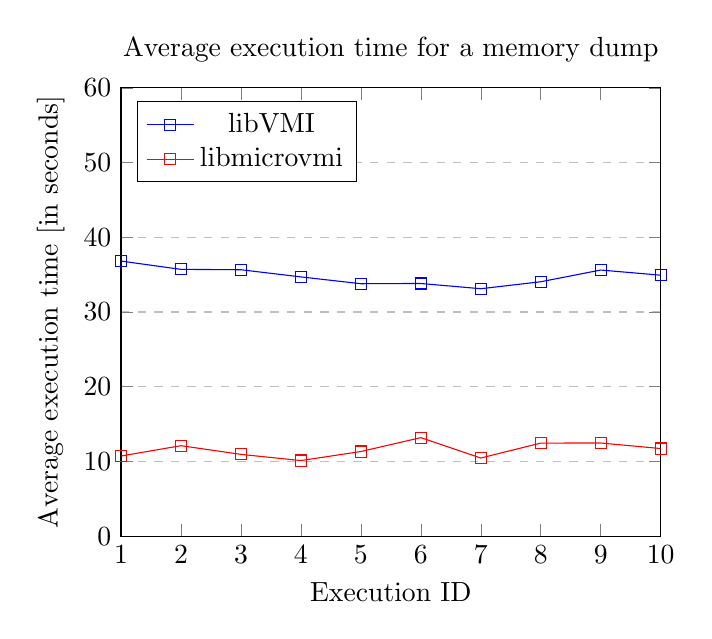
\begin{tikzpicture}
\begin{axis}[
    title={Average execution time for a memory dump},
    xlabel={Execution ID},
    ylabel={Average execution time [in seconds]},
    xmin=1, xmax=10,
    ymin=0, ymax=60,
    xtick={1, 2, 3, 4, 5, 6, 7, 8, 9, 10},
    ytick={0, 10, 20, 30, 40, 50, 60},
    legend pos=north west,
    ymajorgrids=true,
    grid style=dashed,
]

\addplot[
    color=blue,
    mark=square,
    ]
    coordinates {
    (1,36.82)(2,35.71)(3,35.66)(4,34.7)(5,33.79)(6,33.82)(7,33.12)(8,34.05)(9, 35.62)(10, 34.93)
    };
    \addlegendentry{libVMI}
\addplot[
    color=red,
    mark=square,
    ]
    coordinates {
    (1,10.73)(2,12.11)(3,10.95)(4,10.12)(5,11.33)(6,13.19)(7,10.46)(8,12.46)(9, 12.47)(10, 11.73)
    };
    \addlegendentry{libmicrovmi}
    
\end{axis}
\end{tikzpicture}
\newline
\newline
Our measurements showed a noticeable performance advantage in favor of libmicrovmi. 
While it takes libVMI in average 34,82 seconds to perform the memory dump, it only takes 11,56 seconds with libmicrovmi.
This means that libmicrovmi is roughly 3 times faster.
\newline
\newline
\textbf{c) register dump}
\newline
\newline
TO DO's (this is work in progress [WIP] so it doesn't need review)
\begin{itemize}
	\item Summary of what is being measured (reg dump)
	\newline 
	\item Implement register dump for libvmi: There are functions for that in libvmi/driver/xen.c 
	\newline
	\item Implement register dump for libmicrovmi: There is a PR for reading/writing registers 
	\newline
	(https://github.com/Wenzel/libmicrovmi/pull/90). 
	\newline
	This needs to be merged with other changes made to work on our test environment.
	\newline
	\item Use the two reg dumps within the python tool to measure the execution time.
	\newline
	\item Evaluation
	\newline
	\newline
\end{itemize}

\textbf{d) CR3 event}
\newline
\newline
TO DO's (this is WIP so it doesn't need review)
\begin{itemize}
	\item Summary of what is being measured (specific CR3 Event)
	\newline 
	\item Test CR3 event example for libvmi. 
	\newline
	\item Implement cr3 event example for libmicrovmi: The event support is already implemented but not merged in master. There are mulitple PR's which needs to be reviewed.
	\newline
	\item Use the two cr3 event examples within the python tool to measure the execution time. Therefore a specific cr3 event needs to be watched and triggered on the PVM (with another tool).
	\newline
	\item Evaluation
	\newline
	\newline
\end{itemize}

\textbf{d) Total evaluation of the measured times}
\newline
\newline
TO DO's (this is WIP so it doesn't need review)
\begin{itemize}
	\item Evaluate and discuss the measured values
	\newline
\end{itemize}

\section{Conclusion}
Our conclusion is that there are significant differences between libVMI and libmicrovmi. But that doesn’t mean that one library is better than the other. As explained in Section 3.2, they were designed for different use cases and you can tell. While libVMI offers additional features, libmicrovmi tries to stay small, secure and fast. Finally, in Section 3.3, we showed that the speed that Rust and libmicrovmi promise can also be measured. These results promise a bright future, which we will discuss in Section 4.1, for the library.
\newline
\newline
Only the current state of development prevents the widespread use of libmicrovmi. But because it’s still a relatively new low-level interface for virtual machine introspection APIs, new features and fixes are added regularly. Since libmicrovmi is an open source library, everyone can contribute to improve it.

\subsection{Future Work}

At the moment the functionality of libmicrovmi is limited to the x86 architecture, but they plan to offer support for others.
In the future, it will also be possible to use libVMI in conjunction with libmicrovmi. This would combine the functionality and thus the advantages of both libraries.
Therefore, there is already a repository \cite{libmicrovmiintegrationlibvmi} that is currently being worked on.
\newline
\newline
Independently of libmicrovmi, implementing a separate semantic library that uses the provided interface would be an excellent step.
The end goal of the developers of libmicrovmi is to abstract functionality shared by VMI applications with the help of further libraries on top (e.g. the mentioned semantic library).
That would drastically simplify the development of new VMI applications in the future.
\newpage
\bibliographystyle{alpha}
\bibliography{literature}


\appendix


\end{document}
\endinput

